The events in the signal region are used to constrain AQGCs in the effective field theory framework. Nine independent charge conjugate and parity-conserving dimension-8 effective operators are considered~\cite{aqgc_operators}. The dimensionn-8 operators are the following: 
%
\begin{align*}
L_{S,0} &= \left[\left(D_{\mu} \Phi\right)^{\dagger} D_{\nu} \Phi \right] \times \left[\left(D_{\mu} \Phi\right)^{\dagger} D_{\nu} \Phi \right] \\
L_{S,1} &= \left[\left(D_{\mu} \Phi\right)^{\dagger} D^{\mu} \Phi \right] \times \left[\left(D_{\nu} \Phi\right)^{\dagger} D_{\nu} \Phi \right] \\
L_{M,0} &= Tr[\hat{W}_{\mu \nu} \hat{W}^{\mu \nu}] \times \left[ \left(D_{\beta} \Phi\right)^{\dagger} D^{\beta} \Phi \right] \\
L_{M,1} &= Tr[\hat{W}_{\mu \nu} \hat{W}^{\nu \beta}] \times \left[ \left(D_{\beta} \Phi\right)^{\dagger} D^{\mu} \Phi \right] \\
L_{M,6} &= \left[\left(D_{\mu} \Phi\right)^{\dagger}  \hat{W}_{\beta \nu} \hat{W}^{\beta \nu}  D^{\mu} \Phi \right] \\
L_{M,7} &= \left[\left(D_{\mu} \Phi\right)^{\dagger} \hat{W}_{\beta \nu} \hat{W}^{\beta \mu} D^{\nu} \Phi \right ] \\
L_{T,0} &= Tr \left[W_{\mu \nu} W^{\mu \nu} \right] \times Tr \left[W_{\alpha \beta} W^{\alpha \beta} \right] \\
L_{T,1} &= Tr \left[W_{\alpha \nu} W^{\mu \beta} \right] \times Tr \left[W_{\mu \beta} W^{\alpha \nu} \right] \\
L_{T,2} &= Tr \left[W_{\alpha \mu} W^{\mu \beta} \right] \times Tr \left[W_{\beta \nu} W^{\nu \alpha} \right]
\end{align*}
%
Each operator is scaled by the corresponding Wilson coefficient. A nonzero AQGC enhances the production cross section at large masses of the system of the gauge boson pair as can be seen in Figure~\ref{fig:signal2}. Statistical analysis of the event yields is performed with a fit to the mass distribution of the $\PW V$ or $\PZ V$ system. The SM EW production is treated as a background in the statistical analysis. The observed and expected $95\%$ confidence level (C.L.) limits on the AQGC parameters are obtained using a profile likelihood test statistic~\cite{Junk,Read,CLs}. 

The expected yields for different values of the AQGC parameters are obtained using the reweighting feature of the MadGraph package. The expected ratio of the AQGC and MS EW yields as a function of the AQGC parameter is fitted with a parabolic function. This is done for each bin of the mass distribution of the $\PW V$ or $\PZ V$ system as shown in Figure~\ref{fig:aqgc_pol}. The increase of the yield as a function of the anomalous coupling exhibits a quadratic behavior and the fitted parabolic function is used to interpolate between the discrete coupling parameters of the simulated signals.      

\begin{figure*}[htb]
\centering
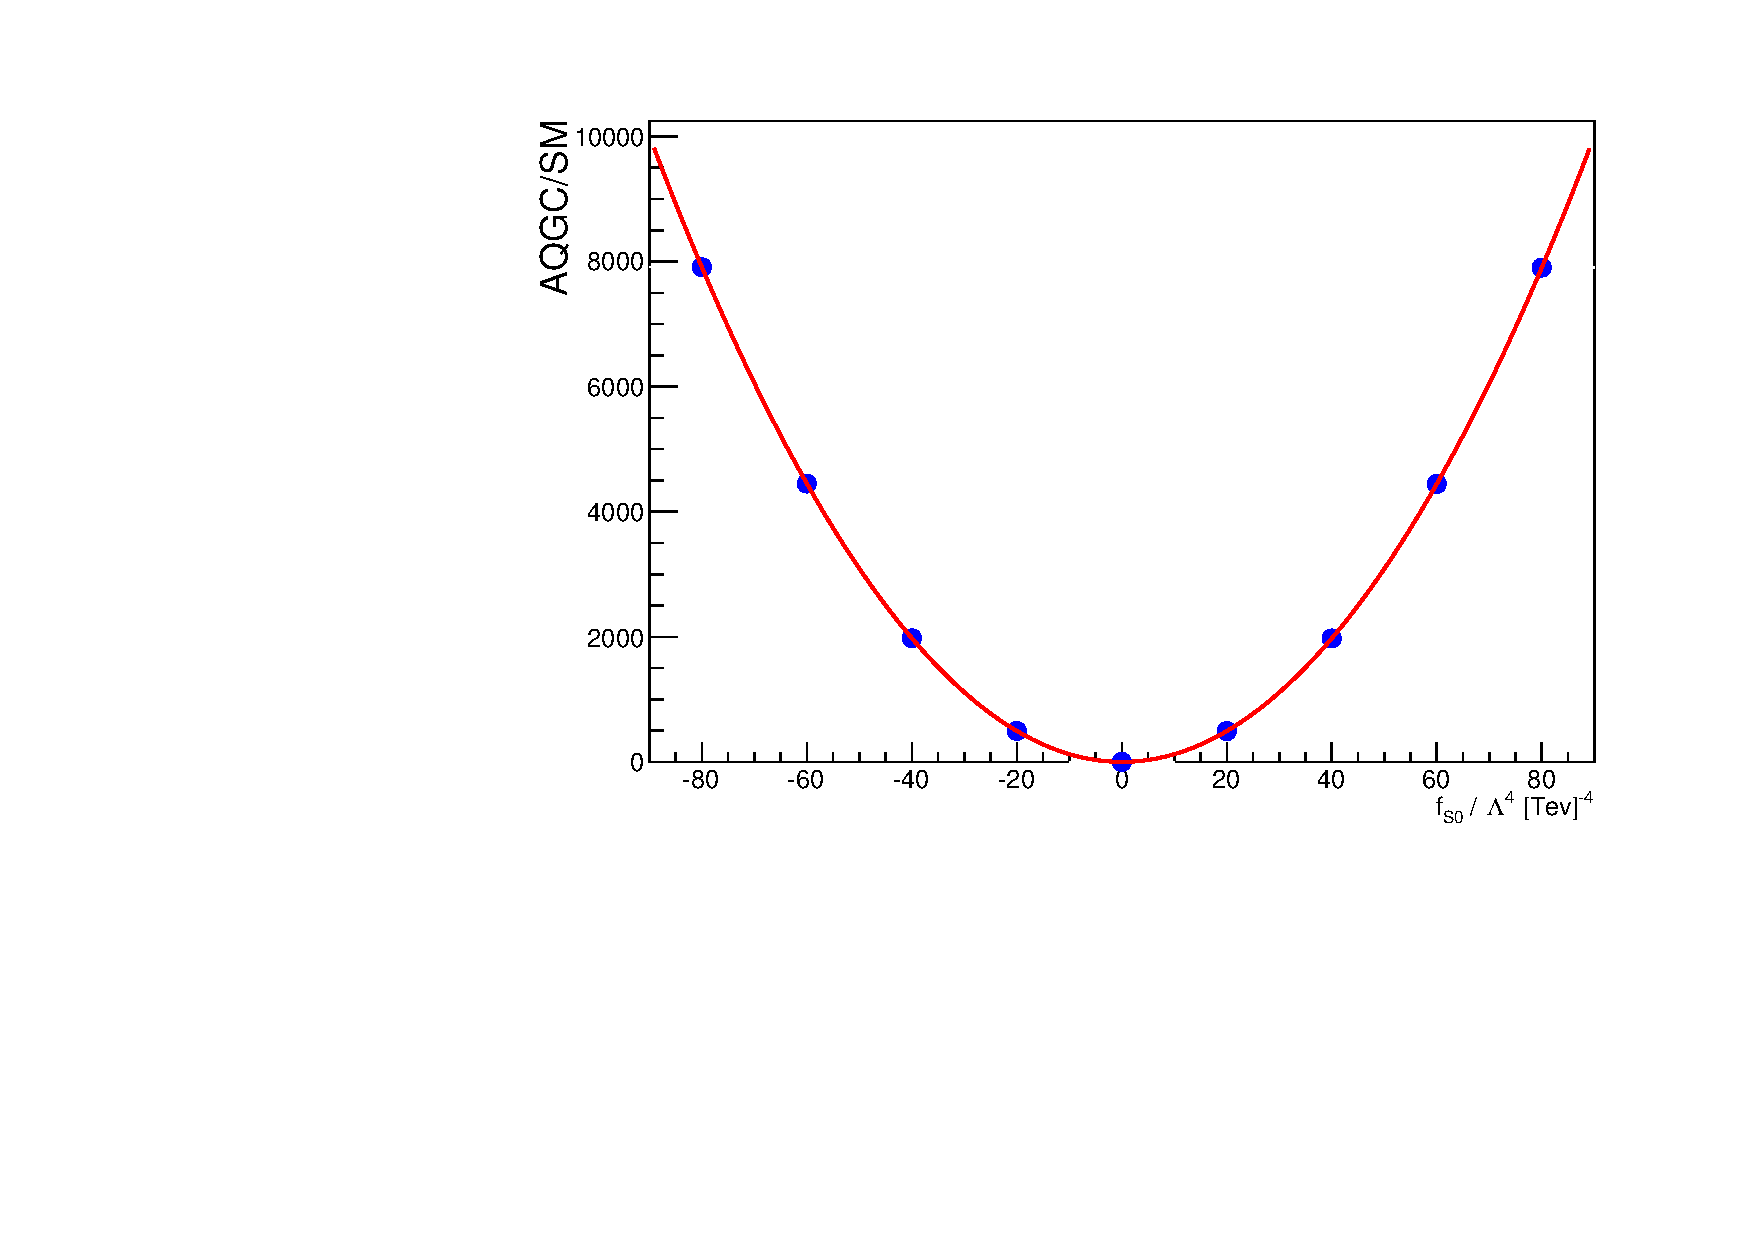
\includegraphics[width=0.45\textwidth]{Plots/plots/aqgc_pol2.pdf}
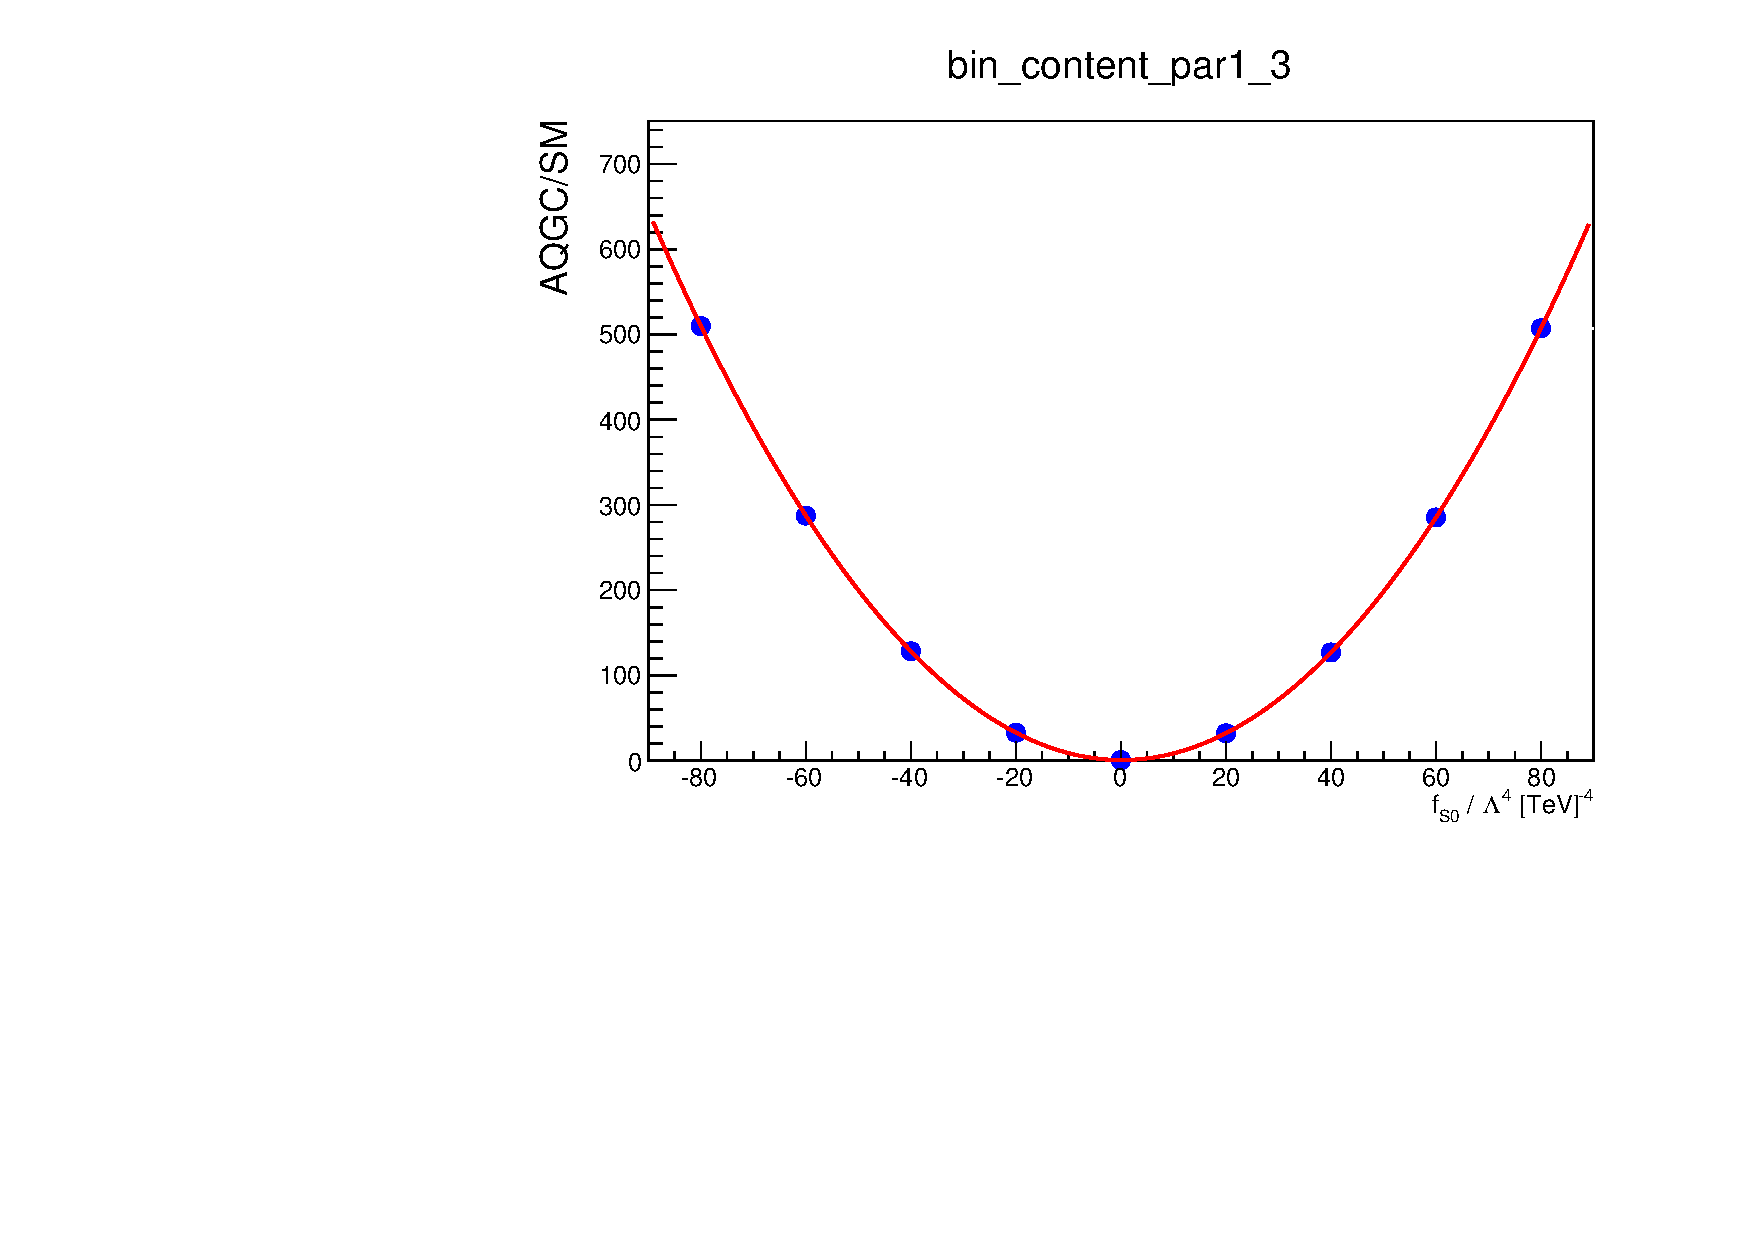
\includegraphics[width=0.45\textwidth]{Plots/plots/aqgc_pol2_bin.pdf}
\caption{Yield ratios of the operator $S0$ and the fitted quadratic interpolation for the most relevant bins used in the statistical analysis. The yields for the mass bins $m_{\PW V}$ = [$2025$,$\infty$] (left) and  $m_{\PW V}$ = [$1550$,$2025$] (right) are shown.}
\label{fig:aqgc_pol}
\end{figure*}

Table~\ref{tab:VBS_aQGC} shows the individual lower and upper limits obtained by setting all other AQGCs to zero using the $\PW V$ final state. The reported values are the most stringent limits reported by the CMS Collaboration previously. The corresponding limits using the $\PZ V$ final state are shown in Table~\ref{tab:VBS_aQGC2}. The combined limits are shown in Table~\ref{tab:VBS_aQGC3}.

% \begin{table}[h!]
% \centering
% \topcaption{
% Observed and expected 95\% C.L. limits on the coefficients
% for higher-order (dimension-8) operators in the effective
% field theory Lagrangian in $\PW V$ final state. 
% }
% \label{tab:VBS_aQGC}
% \begin{scotch}{ccc}
% \ifthenelse{\boolean{cms@external}}{
% & Observed  & Expected  \\
% & limits  & limits \\
% }
% {
% & Observed limits  & Expected limits  \\
% }
% & (\TeV$^{-4}$)   & (\TeV$^{-4}$)   \\
% \hline
% $\mathrm{f_{S0}} / \Lambda^4$  & $[ -X, X]$ & $[ -3.9, 3.9]$ \\
% $\mathrm{f_{S1}} / \Lambda^4$  & $[-X, X]$ & $[-4.9, 4.9]$ \\
% $\mathrm{f_{M0}} / \Lambda^4$  & $[-X, X]$ & $[-0.95, 0.95]$ \\
% $\mathrm{f_{M1}} / \Lambda^4$  & $[ -X, X]$ & $[ -2.8, 2.8]$ \\
% $\mathrm{f_{M6}} / \Lambda^4$  & $[-X, X]$ & $[-1.9, 1.9]$ \\
% $\mathrm{f_{M7}} / \Lambda^4$  & $[-X, X]$ & $[-4.7, 4.7]$ \\
% $\mathrm{f_{T0}} / \Lambda^4$  & $[-X, X]$ & $[-0.16, 0.15]$ \\
% $\mathrm{f_{T1}} / \Lambda^4$  & $[-X, X]$ & $[-0.16, 0.17]$ \\
% $\mathrm{f_{T2}} / \Lambda^4$  & $[-X, X]$ & $[-0.38, 0.38]$ \\
% \end{scotch}
% \end{table}


% \begin{table}[h!]
% \centering
% \topcaption{
% Observed and expected 95\% C.L. limits on the coefficients
% for higher-order (dimension-8) operators in the effective
% field theory Lagrangian in $\PZ V$ final state. 
% }
% \label{tab:VBS_aQGC2}
% \begin{scotch}{ccc}
% \ifthenelse{\boolean{cms@external}}{
% & Observed  & Expected  \\
% & limits  & limits \\
% }
% {
% & Observed limits  & Expected limits  \\
% }
% & (\TeV$^{-4}$)   & (\TeV$^{-4}$)   \\
% \hline
% $\mathrm{f_{S0}} / \Lambda^4$  & $[ -X, X]$ & $[ -28, 28]$ \\
% $\mathrm{f_{S1}} / \Lambda^4$  & $[-X, X]$ & $[-22, 22]$ \\
% $\mathrm{f_{M0}} / \Lambda^4$  & $[-X, X]$ & $[-4.8, 4.8]$ \\
% $\mathrm{f_{M1}} / \Lambda^4$  & $[ -X, X]$ & $[-15, 15]$ \\
% $\mathrm{f_{M6}} / \Lambda^4$  & $[-X, X]$ & $[-9.6, 9.6]$ \\
% $\mathrm{f_{M7}} / \Lambda^4$  & $[-X, X]$ & $[-23, 23]$ \\
% $\mathrm{f_{T0}} / \Lambda^4$  & $[-X, X]$ & $[-0.90, 0.90]$ \\
% $\mathrm{f_{T1}} / \Lambda^4$  & $[-X, X]$ & $[-0.92, 0.93]$ \\
% $\mathrm{f_{T2}} / \Lambda^4$  & $[-X, X]$ & $[-2.1, 2.2]$ \\
% \end{scotch}
% \end{table}

% \begin{table}[h!]
% \centering
% \topcaption{
% Observed and expected 95\% C.L. combined limits on the coefficients
% for higher-order (dimension-8) operators in the effective
% field theory Lagrangian in $\PW V$ and $\PZ V$ final states. 
% }
% \label{tab:VBS_aQGC3}
% \begin{scotch}{ccc}
% \ifthenelse{\boolean{cms@external}}{
% & Observed  & Expected  \\
% & limits  & limits \\
% }
% {
% & Observed limits  & Expected limits  \\
% }
% & (\TeV$^{-4}$)   & (\TeV$^{-4}$)   \\
% \hline
% $\mathrm{f_{S0}} / \Lambda^4$  & $[ -X, X]$ & $[ -3.9, 3.9]$ \\
% $\mathrm{f_{S1}} / \Lambda^4$  & $[-X, X]$ & $[-4.8, 4.8]$ \\
% $\mathrm{f_{M0}} / \Lambda^4$  & $[-X, X]$ & $[-0.94, 0.94]$ \\
% $\mathrm{f_{M1}} / \Lambda^4$  & $[ -X, X]$ & $[ -2.8, 2.8]$ \\
% $\mathrm{f_{M6}} / \Lambda^4$  & $[-X, X]$ & $[-1.9, 1.9]$ \\
% $\mathrm{f_{M7}} / \Lambda^4$  & $[-X, X]$ & $[-4.7, 4.7]$ \\
% $\mathrm{f_{T0}} / \Lambda^4$  & $[-X, X]$ & $[-0.16, 0.15]$ \\
% $\mathrm{f_{T1}} / \Lambda^4$  & $[-X, X]$ & $[-0.16, 0.17]$ \\
% $\mathrm{f_{T2}} / \Lambda^4$  & $[-X, X]$ & $[-0.38, 0.38]$ \\
% \end{scotch}
% \end{table}

% The exclusion limits on the charged Higgs  $\sigma_\mathrm{VBF}(\PHpm) \mathrm{B}(\PHpm\to \PW\Z)$
% at 95\% confidence level as a function of $m(\PHpm)$,
% assuming a small intrinsic width for $\PHpm$, are also planned to be included in the paper.
% We are waiting for the Doubly charged Higgs boson signal samples to be produced. We plan to include this interpretation by the approval. The coupling depends on $m(\PHpm)$ and the parameter $s_{\PH}$, where $s_{\PH}^2$ denotes the fraction of the $\W$ boson mass squared generated by the vacuum expectation value of the triplets. The model-independent exclusion limits can be used to constrain the $s_{\PH}$-$m(\PHpm)$ plane by using the predicted cross sections at NNLO accuracy in the GM model~\cite{Zaro:2002500}. 

%In Fig.~\ref{fig:limits} (\cmsRight), the excluded $s_{\PH}$ values as a function of $m(\PHpm)$ are shown.

%are shown in Fig.~\ref{fig:limits} (left). 
%The limits given here are placeholders and will improve approximately by a factor of three by including the doubly charged Higgs boson contribution.

%\begin{figure}[htbp]
%\centering
%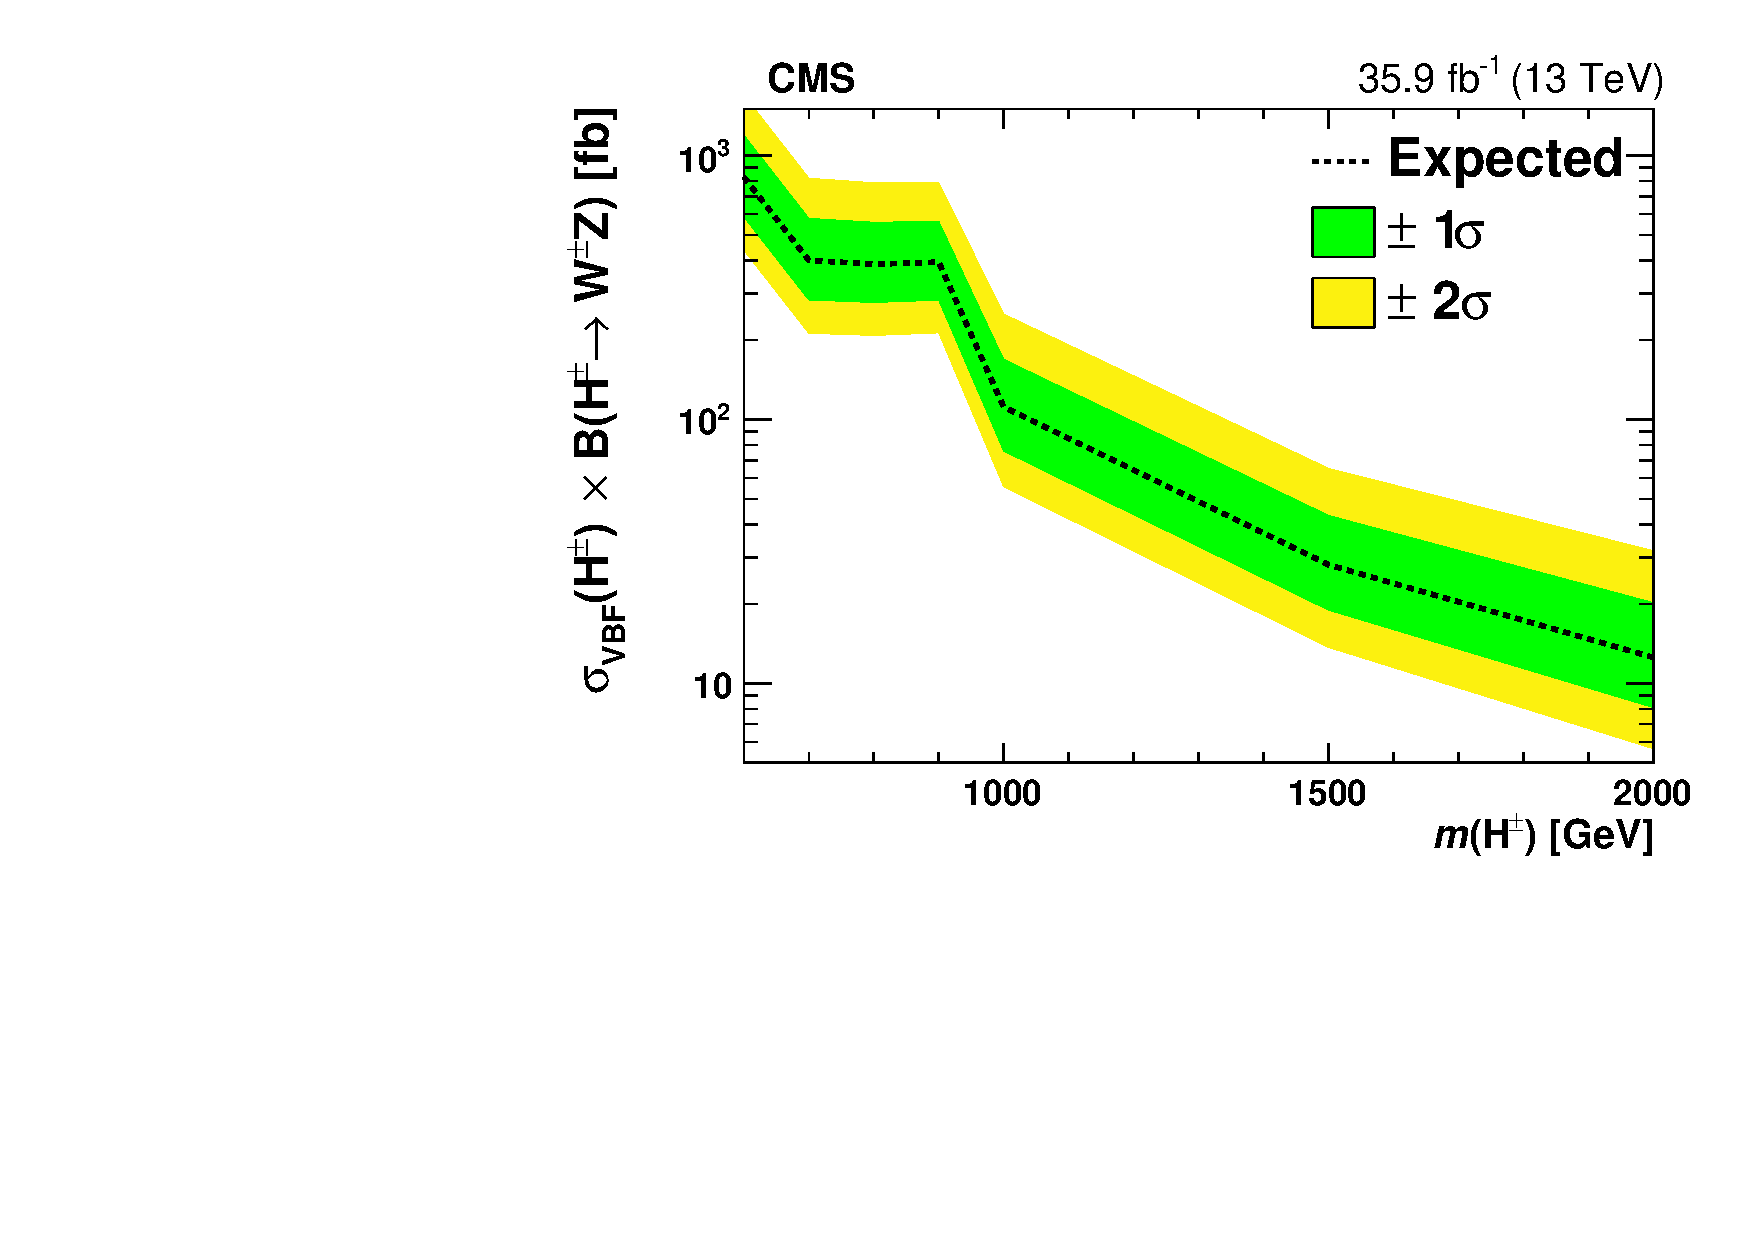
\includegraphics[width=0.9\textwidth]{Plots/plots/limits_independent.pdf}
%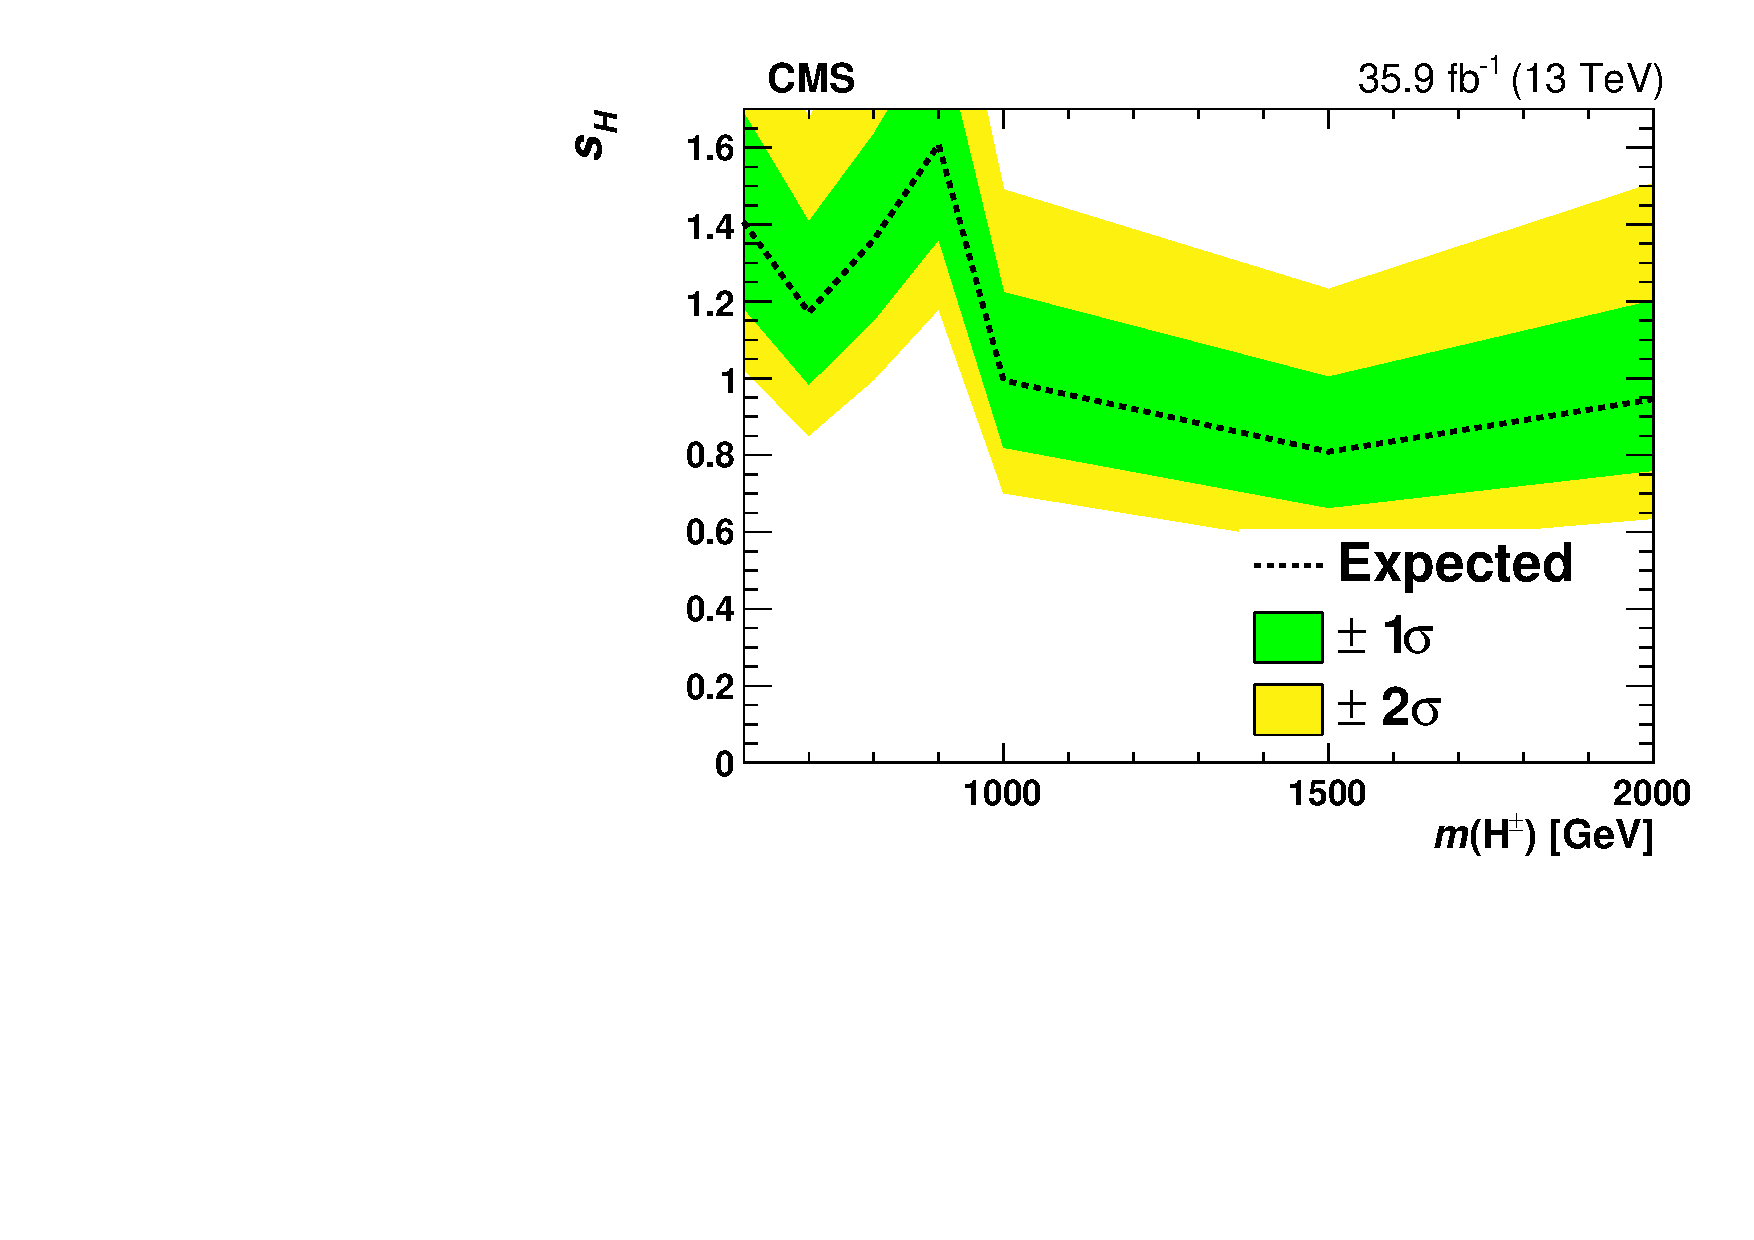
\includegraphics[width=0.9\textwidth]{Plots/plots/limits_model_dependant.pdf}
%\caption{Expected and observed exclusion limits at 95\% confidence
%level as a function of $m(\PHpm)$ for $\sigma_\mathrm{VBF}(\PHpm) \, \mathcal{B}(\PHpm\to \PW\Z)$ (\cmsLeft) and on the ratio of vacuum expectation values in the GM model (\cmsRight). 
%The blue shaded area covers the theoretically not allowed parameter space~\cite{Zaro:2002500}.
%}
%\label{fig:limits}
%\end{figure}
